\documentclass[tikz,border=10pt]{standalone}
\usepackage{tikz}
\usetikzlibrary{positioning}

\begin{document}

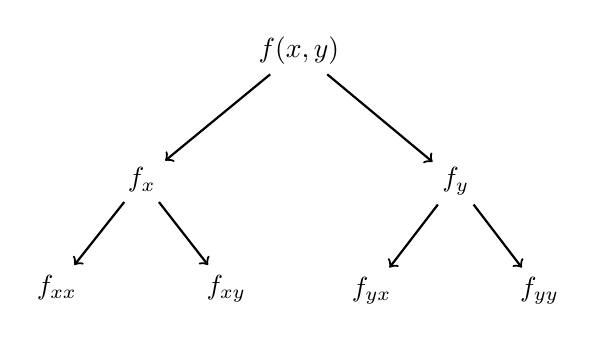
\begin{tikzpicture}[node distance=15mm, arrow/.style={->, thick}, scale = 2]

%prva razina slike
\node (f) {$f(x,y)$};

%druga razina slika
\node (fx) [below left=of f] {$f_x$};
\node (fy) [below right=of f] {$f_y$};

%treća razina slike
\begin{scope}[node distance=8mm and 4mm]
    \node (fxx) [below left=of fx] {$f_{xx}$};
    \node (fxy) [below right=of fx] {$f_{xy}$};
    \node (fyx) [below left=of fy] {$f_{yx}$};
    \node (fyy) [below right=of fy] {$f_{yy}$};
\end{scope}

%strelice od f prema parcijalnim derivacijama
\draw[arrow] (f) -- (fx);
\draw[arrow] (f) -- (fy);

%strelice od parcijalnih derivacije prema derivacijama drugog reda
\draw[arrow] (fx) -- (fxx);
\draw[arrow] (fx) -- (fxy);
\draw[arrow] (fy) -- (fyx);
\draw[arrow] (fy) -- (fyy);

\end{tikzpicture}

\end{document}
